\chapter{Introduction}\label{chap:chapter1}

The work presented in this thesis is part of an industry linked PhD under the Center for Transforming Maintenance Through Data Science (CTMTDS), a center comprised of both academic and industry partners. One of the centre's goals is to develop methods that support reliability engineers in managing uncertainty during the maintenance decision making process--i.e. how and when they should maintain an asset based on their understanding of the asset and the available data. As part of the industry linked PhD, I spent a reasonable period working on industry placement projects (900 hours in total between two different industry partners) to outlining research topics that are not only novel in an academic sense but also facilitate a greater use of robust statistical modelling by reliability practitioners when making maintenance decisions in the mining and mineral processing industry.

It was apparent from my placement time that there is a disconnect between the reliability modelling literature and the methods used by reliability practitioners in the mining and mineral processing industry, often referred to as a theory-practice gap. There are many well-established models for reliability data such as the Weibull distribution for lifetime data, or stochastic process models for degradation data. There is also a desire by mine, processing plant, and refinery operators to use these models since once an asset is put into service, completely new information becomes available, which can be utilised so that operators can make better maintenance decisions based on the specific reliability characteristics of their assets, rather than estimates from the manufacturer \citep{jardine2013}. But this new information is collected in the field (where there are many sources of noise) and within large companies (where it is difficult to regulate data collection practice and where there is a constant trade-off between cost, safety, and time versus the quality and amount of data collected). This results in unique observational processes that need their own sophisticated modelling approaches before reliability practitioners in the mining and mineral processing industry can take advantage of the well-established reliability models in the literature. Two examples of issues confronting reliability engineers that I tackle in this thesis are 1) obtaining reasonable estimates of lifetime distributions when lifetime data are heavily censored due to the pre-emptive replacement of assets or limitations of data recording and 2) forecasting complex degradation processes with noisy and sparsely observed condition monitoring data. In this thesis, I show novel expansions of some of the well-established reliability methods through the Bayesian model building approach \citep{gelman_workflow_2020} and demonstrate how they can be applied to observational industry data sets (from overland iron ore conveyors) provided by the centre's industry partners.

The Bayesian paradigm became a strong backbone of this thesis because Bayesian methods provide a formal structure to build complicated models and incorporate multiple sources of information, such as domain expert knowledge \citep{meeker2022}. Furthermore, the resulting full posterior distribution obtained through Bayesian analysis allows us to easily produce estimates and uncertainty intervals for complicated functions of the model parameters \citep{meeker2022}, which is extremely useful for propagating uncertainty through a decision-making process. While there is a well-developed subfield of Bayesian analysis in the reliability literature \citep{hamada2008, meeker2022}, the Bayesian framework is underutilised in industry. This underutilisation is most likely because, for most cases, inference must be obtained through Monte Carlo simulation, and in the past, this has meant constructing Markov Chain Monte Carlo (MCMC) algorithms by hand. However, the recent increase in popularity of Bayesian methods has led to the development of flexible and accessible probabilistic programming languages such as BUGS \citep{lunn2012}, JAGS \citep{plummer2003} and Stan \citep{Stan2022}, which in many cases alleviate the analyst form the need to construct bespoke MCMC algorithms. The result is a newfound ability to fit and explore complex models relatively quickly and simply.  

To harness these new aspects of statistical modelling more effectively, the applied Bayesian statistical community has started to develop a more rigorous workflow for building, fitting, checking, and comparing Bayesian models. Throughout this thesis, I clearly emphasise the components of this workflow and demonstrate them in a reliability setting. In doing so, I hope this thesis may also be used as a template for other maintenance decision-making problems in the field.

The rest of this chapter provides a general background for the rest of the thesis. First, in \textit{section}~\ref{sec:decisions}, I provide some context around maintenance decision-making in the mining and mineral processing industry. Then, in \textit{section}~\ref{sec:reliability}, I give a high-level overview of reliability modelling and how it informs maintenance decisions. \textit{Section}~\ref{sec:Bayesian-methods} outlines Bayesian methods and the key components of the Bayesian model building workflow, which will be a strong thematic thread throughout the remainder of the thesis. Finally, in \textit{section}~\ref{sec:thesis-structure}, I lay out the structure of the thesis.

\section{Maintenance decision making}
\label{sec:decisions}

The maintenance of an asset can be considered as \textit{"all activities aimed at keeping an \{asset\} in, or restoring it to, the physical state considered necessary for the fulfilment of its production function"} \citep{geraerds1985}. In other words, the main objective of maintenance actions is to fix/replace an asset's components to ensure that the asset can perform its desired duty at an acceptable level of performance. In this context, the only consideration when deciding when to maintain the asset is whether or not the asset is performing its duty at an acceptable level. However, in reality, the maintenance of any single asset exists in the much larger context of a company \citep{jardine2013}. There are finite resources, budget, and time that can be allocated to the maintenance of any specific asset, and some assets are more critical to production than others. This "big picture" management of an asset's maintenance is what we refer to as asset health management. It is in this bigger context that reliability engineers and planners must make their decisions about how and when to maintain an asset. Asset health management requires foresight, planning, and--most importantly--risk management.

Maintenance strategies help to roughly allocate resources and plan maintenance schedules ahead of time. There are three general strategies: reactive, preventative, and predictive maintenance \citep{jardine2013}. We provide a more detailed overview of these strategies a little later. An asset can have different strategies for its different components, and typically, the choice of strategy is dictated by how critical the component is, how expensive it is, and what type of data we can collect. But even with a maintenance strategy, once an asset is put into service, we start to gather new data that can be used to refine/inform the maintenance strategy. For instance, \textit{Chapter}~\ref{chap:chapter4} uses failure time data to inform the timing of a bulk-replacement strategy.

\subsubsection*{Reactive vs Preventative vs Condition-based maintenance strategy}

The simplest replacement strategy is a reactive maintenance strategy, whereby components are only replaced once they fail \citep{heng2009}. Reactive strategies are used mostly for non-critical components. They are not typically used for mechanical components in mining because the cost due to lost production when an asset fails unexpectedly is orders of magnitude greater than the cost of planned maintenance. On the other hand, a preventative replacement strategy is when components are replaced pre-emptively after a designated period of time or operation. This proactive approach to maintenance is suitable for cheap components whose reliability decreases with time. i.e. components that wear out (most mechanical components). A downfall of preventative maintenance is that it can result in overmanning assets, which is a waste of money and resources. If a component is costly and critical, and it is possible to monitor its condition somehow, then a condition-based maintenance strategy should be used. Condition-based maintenance balances using as much of the component's useful life as possible with the reduced risk of lost production by monitoring the degradation of a component and replacing it when it gets to a predetermined, unacceptable level.

There are obvious ways in which statistical modelling can inform preventative and condition-based strategies. Implementing a preventative replacement strategy requires choosing a pre-emptive time to replace the component. The better the choice, the better the strategy will perform. A component's specific environmental and operating conditions affect its reliability \citep{meeker2022}. So, if it is possible to use data to "tune" the replacement time to the component's reliability under the specific operating conditions, then the preventative policy will be more successful. Condition-based strategies, on the other hand, are more useful if we can forecast the degradation through time to predict the failure time (useful life) of the component. More detailed and accurate forecasts will result in better maintenance plans and reduce the risk of an unexpected failure. In both cases, the more accurately we can estimate the reliability quantities, the better the strategies will perform. We can estimate these quantities and manage uncertainty around the estimates by fitting reliability models to data.

\section{Reliability modelling}
\label{sec:reliability}

In the engineering context, reliability is the "ability of an item to perform a required function under given conditions for a given time interval" \citep{ISO_14224_2016}. This definition is very closely tied to the definition of maintenance actions in \textit{Section}~\ref{sec:decisions}; maintenance actions are to ensure reliability. In the reliability modelling context, the definition of reliability is slightly different. It is the "probability for an item to perform a required function under given conditions over a given time interval $(0, t)$" \citep{ISO_12489_2013}. In other words, it quantifies the engineering definition of reliability as a probability that a unit will not fail before $t$, that is, $P(T > t)$. Here, time $t$ can be calendar time, operating time, or some other exposure, such as loading cycles, distance travelled, or throughput \citep{lee2006}.

The modelling definition of reliability focuses on binary outcomes (i.e., success/failure data) for a set time interval \citep{hamada2008}. But typically, we have more detail in data and instead want to estimate the reliability at all values of $t = [0, \infty)$. This representation is the reliability function, $R(t)$. The reliability function can alternatively be represented as its complement, $P(T \le t)$, the cumulative failure time distribution, $F(t)$ \citep{meeker2022}. Reliability analysis aims to estimate these functions from data. Two general approaches are taken, depending on the type of observations available: Lifetime modelling (also referred to as failure time models) and degradation models (sometimes referred to as repeat repeated-measures degradation models).

\paragraph*{Lifetime modelling} 

The most common form of reliability data are lifetime data. These are the recorded installation and failure times of units in operation. Lifetime modelling, therefore, aims to estimate the failure time distribution from lifetime data. These lifetime data can come from repeated failures of an asset or the lifetimes of a population of assets. The estimated failure time distribution from lifetime analysis allows the analyst to make general statements about the reliability of a population conditional on some exposure time $t$ and sometimes on covariates \cite{moore2016}. However, it is common for reliability datasets to be limited in size or the number of observed failures \citep{meeker2022}. For example, a particular asset may only have a small number of failures, or in a population of highly reliable assets, only a few may fail over the period of observation. In these cases, the data are not very informative. To combat a lack of information, the analyst can either supplement the analysis with other sources of information (which we elaborate on in \textit{Part}~\ref{part:one}) or use a degradation model if they have access to measurements of the degradation process that drives failure (the focus of \textit{Part}~\ref{part:two}).

\paragraph*{Degradation modelling} 

Using an example from \citet{meeker2022}, consider the case that in a lifetime dataset, only two out of one hundred units fail. In this case, the ninety-eight units that did not fail provide no information about how close they were to failure. If, in addition, there are repeated measurements of the level of the degradation mechanism that drives the failure, then degradation analysis allows us to look inside the other ninety-eight units and, more precisely, estimate the failure time distribution. In fact, degradation modelling can be used to derive failure time distributions if there are no failures or even for a single unit that has not yet failed (\textit{Part}~\ref{part:two}). The connection between degradation models and failure time distribution is well explored \citep{lu1996,bae2007,meeker2022,lawless2004}, and the connection is typically made using soft failure.

Soft failure is defined by a predetermined threshold of degradation, compared to hard failures, which are when the component can no longer operate \citet{hamada2008}. Hard failures are more stochastic in nature, making them more risky, hence why soft failure is often used. However, regardless of whether a soft or hard failure definition is used, when the failure time distribution is derived from a degradation model, it is important to note that the distribution is conditional on the particular degradation failure mode we are modelling.

Statistical degradation models can be divided into general path models or stochastic process models \citep{pandey2006, si2011}. General path models assign a functional form to the degradation path of a unit, typically a theoretically motivated function such as in \citep{robinson2000}. This method assumes that the functional form can sufficiently represent the underlying degradation and that measurement error can completely account for any deviations in measurements from this fixed path. Heterogeneity between units can be added through regression/random effects \citep{robinson2000}. On the other hand, stochastic processes do not assume a fixed path \citep{pandey2006}. In Stochastic processes, the jumps in degradation are modelled as random variables, meaning that they account for random variation in the degradation process over time. The stochastic process model we focus on is the Gamma process, like in \citep{lawless2004}. A rough comparison of the two methods is made in \citep{zhi-sheng2015}; however, no comprehensive comparisons have been explored. This is an open-ended research question, but we will not tackle it in this thesis.

\section{Industry Examples}
\label{sec:industry-data}

In this thesis, I show two examples of industry problems. Both problems relate to the components of an overland iron ore conveyor. One example is a preventative maintenance problem, and the other is a condition-based one. In \textit{Part}~\ref{part:one} of the thesis, I look at the preventative replacement of idlers. Whereas in \textit{Part}~\ref{part:two} I focus on forecasting the degradation of the conveyor belting to inform condition-based decisions. The two components are shown in \textit{Figure}~\ref{fig:belt_and_frame}.

\begin{figure}[h]
  \centering
  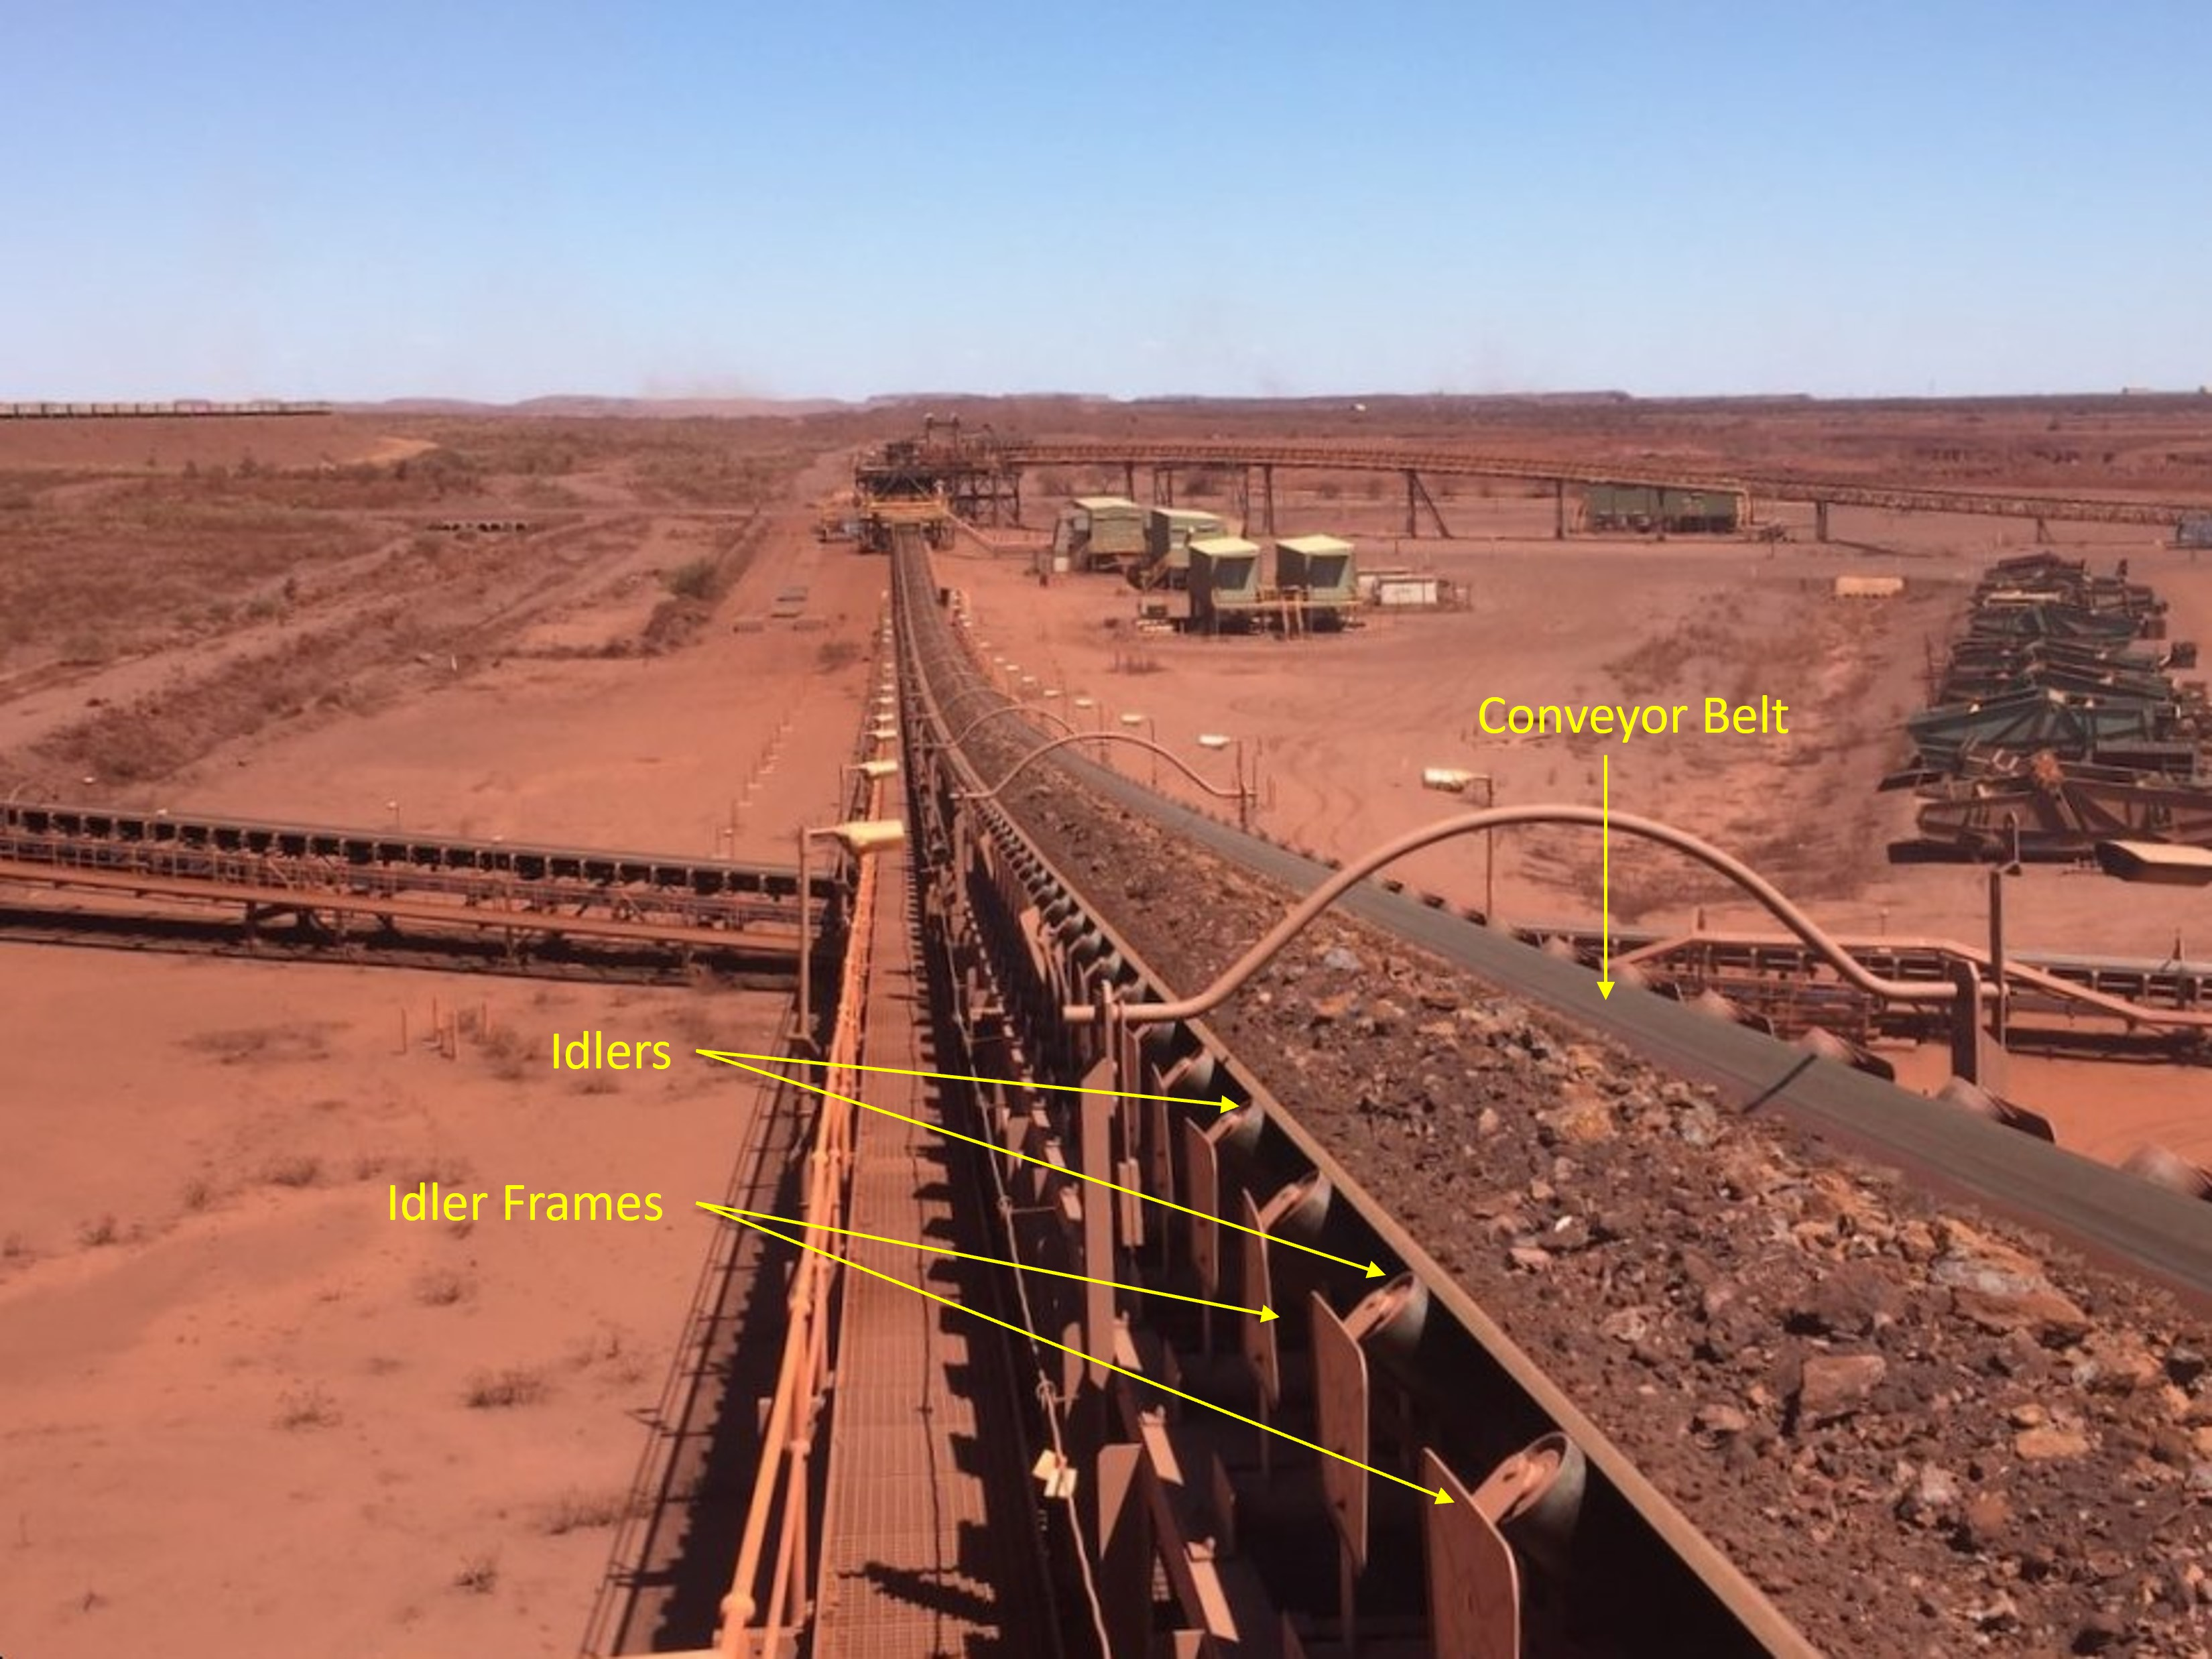
\includegraphics[width=1\textwidth]{./figures/cvr_example_edit_annotation.jpg}
  \caption{An annotated image of an overland iron ore conveyor \citep{australianmining2020} showing the belting, idlers, and idler frames.}
  \label{fig:belt_and_frame}
\end{figure}

\paragraph*{Idlers}

Idlers (sometimes called rollers) support the weight of the belt and ore. They are relatively cheap components, and there can be hundreds or thousands of them on a single conveyor. Idlers are organised in frames, usually consisting of three idlers: one central idler directly under the belt and two wing idlers supporting the sides of the belt to create the cupped shape. The idlers and idler frames are shown in \textit{Figure}~\ref{fig:belt_and_frame}. Idlers are mechanical components and, therefore, wear out with operation. When an idler fails, it does not cause a direct impact on production; however, failed idlers can damage the belt, and damage to the belt results in major downtime. Reliability engineers need to manage the replacement of the idlers to minimise the risk of them failing and damaging the belt while simultaneously minimising the maintenance cost. It is not yet financially viable to monitor the condition of all idlers on a single conveyor, let alone all conveyors on a mine site. Therefore, a preventative maintenance strategy is used.

\begin{figure}[h]
  \centering
  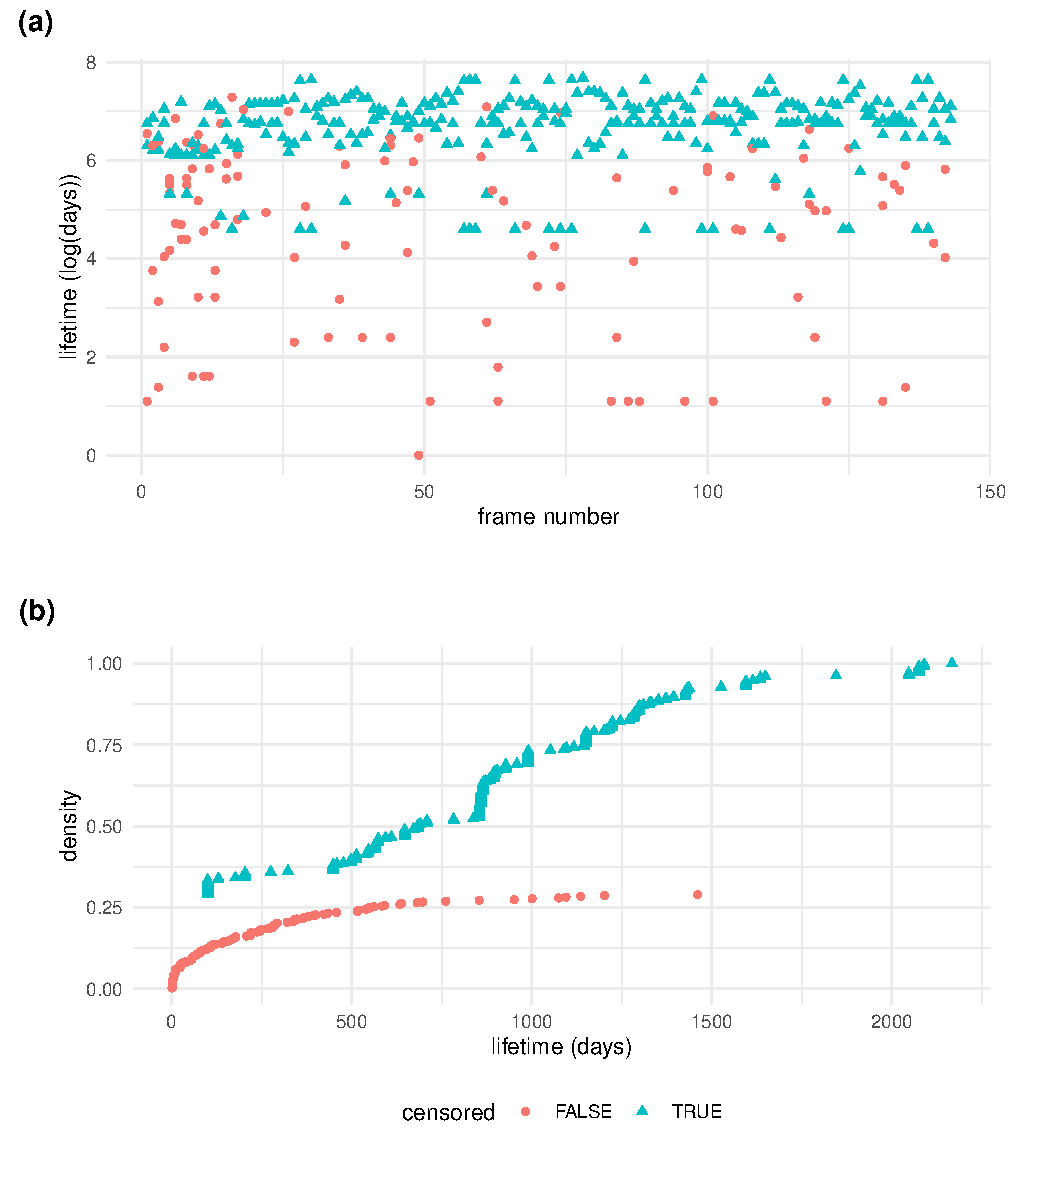
\includegraphics[width=1\textwidth]{./figures/idler_data_desc.pdf}
  \caption{(a) frame lifetimes. (b) eCDF of lifetimes}
  \label{fig:idler-data}
\end{figure}

Survival data of the idlers--derived from installation and replacement times--can be used to inform the preventative maintenance strategy for the idlers. Unfortunately, the failure data is usually only reliably recorded down to the frame number level, not the position of the idler in the frame. However, when one of the idlers in a frame fails, usually all the idlers in that frame are replaced, meaning that we can model the reliability of the idler frames to inform the preventative maintenance strategy. An example data set is shown in \textit{Figure}~\ref{fig:idler-data}~\textit{a}. The figure shows the frame lifetimes for a single overland conveyor over six years. Because idlers are long-lasting components and also because they are preventatively replaced, there are many cases where we do not observe the entire lifetime of an idler either because it had not failed by the time we stopped observing it or it was pre-emptively replaced. These partially observed lifetimes are censored lifetimes and are shown in blue in \textit{Figure}~\ref{fig:idler-data}~\textit{a}. We discuss censoring in more detail in \textit{Part}~\ref{part:one}. \textit{Figure}~\ref{fig:idler-data}~\textit{b} shows the non-censored and censored lifetimes plotted cumulatively. In the ordered plot, we can see that many of the shorter lifetimes are fully observed, while most long lifetimes are obscured by censoring.

\paragraph*{Belt}

The belt of an overland conveyor is much more costly to replace (both in terms of time and money). Furthermore, if the belt fails, then major downtime is inevitable. Over time, the constant loading of ore onto the belt wears away a protective topcoat of rubber, exposing the structural components of the belt to the risk of being damaged by the ore. To ensure the structural integrity of the belt, Engineers stop the belt occasionally to take ultrasonic-thickness (UT) measurements of the topcoat and make sure that it is thick enough to provide adequate protection. An example of the UT data is shown in \textit{Figure}~\ref{fig:belt_wear_ut}.

Engineers use these UT measurements to estimate the soft failure time of the belt and plan its replacement, i.e. forecast when the top coat will no longer be thick enough to protect the belt. However, forecasting the wear of the belt to inform decisions requires robust statistical modelling to properly quantify the many different sources of uncertainty, which can be done in the Bayesian framework.

\begin{figure}[h]
  \centering
  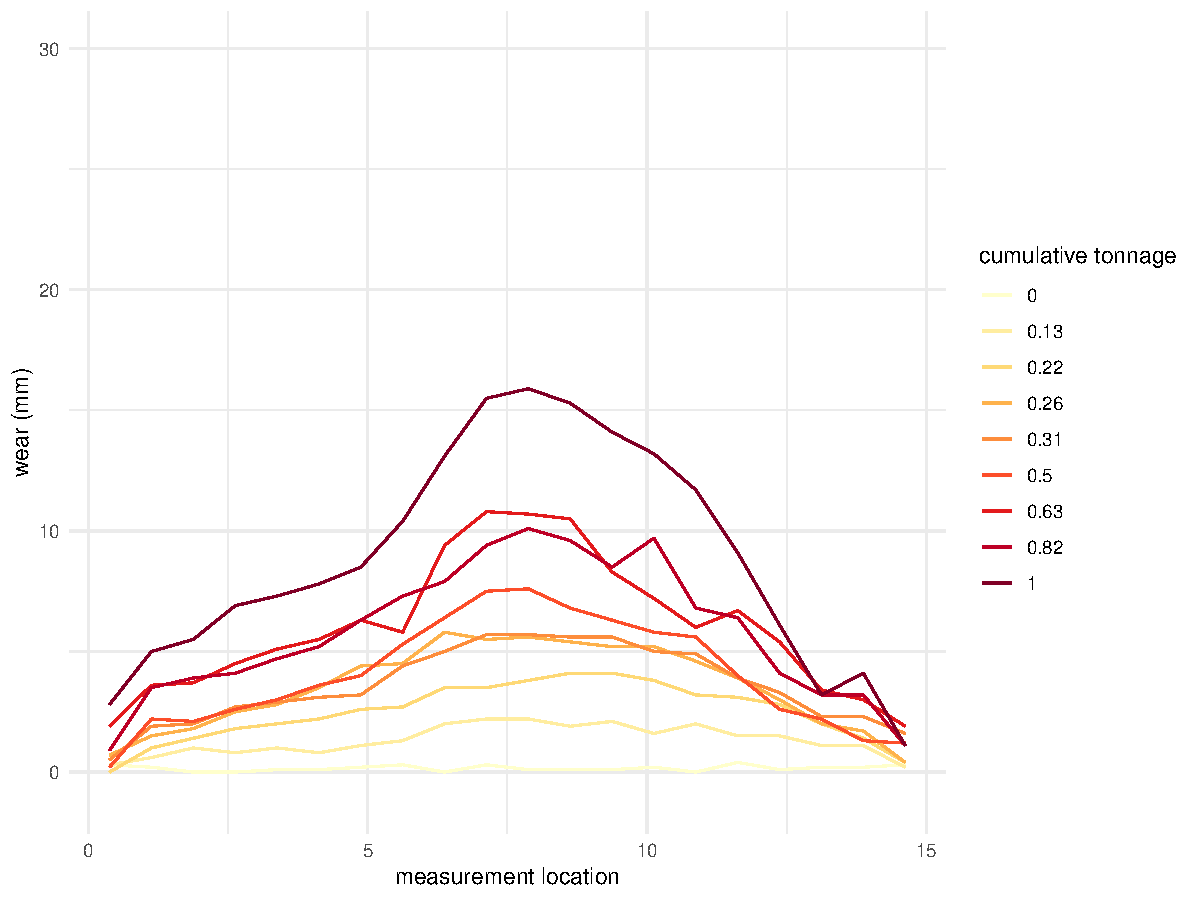
\includegraphics[width=1\textwidth]{./figures/belt_wear_ut.pdf}
  \caption{Belt UT measurement data.}
  \label{fig:belt_wear_ut}
\end{figure}

\section{Bayesian reliability modelling}
\label{sec:Bayesian-methods}

In the Bayesian statistical framework, probabilities are subjective statements about our uncertainty. In a Bayesian analysis, we aim to construct probability statements about parameters of interest, $\theta$, conditioned on the data $y$ and (implicitly) on the values of covariates \citep{BDA2020}. That is, we wish to obtain $P(\theta|y)$, known as the posterior distribution. To do this, Bayesian inference relies on Bayes rule,
\begin{equation}
  P(\theta|y) = \frac{P(y|\theta)P(\theta)}{P(y)},
\end{equation}
where $P(y|\theta)$ is the likelihood of the data conditional on $\theta$, $P(y)$ is the marginal distribution of the data, and $P(\theta)$ is the prior distribution of the parameters. The prior distribution encodes our belief about the parameters before observing the data and, therefore, encodes any additional information that we may have about the phenomenon we are modelling, either from historical data or domain expertise. Alternatively, we can write the un-normalised posterior as
\begin{equation}
  P(\theta|y) \propto p(y|\theta)P(\theta).
\end{equation}

In practice, however, the posterior distribution is rarely available in closed form, and we need to simulate draws from the posterior distribution using Markov chain Monte-Carlo (MCMC) methods to perform inference. There are several powerful and flexible probabilistic programming languages, such as STAN, which allow us to easily implement MCMC algorithms for complex model structures.

\paragraph*{Bayesian workflow}

Surrounding Bayesian inference is a larger workflow of good statistical practice. Just as there is good practice for statistical modelling, the applied Bayesian community has developed its own workflow tailored to the specifics of Bayesian analysis \citep{gelman_workflow_2020}, the main components of which focus on model construction, drawing from the posterior using MCMC methods and diagnosing issues with computation, sense checking the model with simulated data, evaluating and using the posterior distribution, and comparing and expanding models. Here, I give a very high-level overview of the components in the workflow most relevant to this thesis. See \citep{gelman_workflow_2020} for an in-depth description of a Bayesian workflow. The components of this workflow that I use within this thesis are; conditional modelling, prior predictive checking, sampling and diagnostics, posterior predictive checking and posterior inference, and model comparison.

\paragraph*{Model specification}

The first step of any Bayesian analysis is to postulate a joint probability distribution for the model. For complicated processes, this first step can be simplified by using a Bayesian Hierarchical (multi-level) Modelling approach, which uses the fundamental notion of the \textit{the law of total probability}, $P(A, B, C) = P(A|B, C) P(B|C) P(C)$, to decompose a complicated joint probability into a string of simpler conditional probabilities \citep[p.~13]{wikle_2019}. \citet{Berliner_1996} proposed Bayesian Hierarchical Modelling (BHM) as a way of studying an underlying latent process by breaking the joint probability of the data, process, and parameters down into three sub-models;
\begin{align*}
  p(\text{data}, \text{process}, \text{parameter}) = & p(\text{data}| \text{process}, \text{parameter}) && \text{data model} \\
  & p(\text{process}| \text{parameter}) && \text{process model} \\
  & p(\text{parameter}) && \text{parameter model}
\end{align*}
The first level is the data model, $p(\text{data} | \text{process}, \text{parameter})$, which describes the observation process. The second level in the hierarchy is the process model, $p(\mbox{process} | \text{parameter})$. It describes the underlying process that is of scientific interest. The third level in the hierarchy, $p(\text{parameter})$, is the parameter model, and in a Bayesian setting refers to the prior distribution. Each of these different levels in the hierarchy can also be made up of smaller constituent conditional models. \citet{cressie_2011} advocate using the BHM approach for studying underlying latent spatial and spatio-temporal processes, but the same general approach is used to break down models for nested data structures under the term multi-level modelling \citep{BDA2020}. 

In the last level of this hierarchical structure, the prior distribution summarizes any a priori beliefs the analyst has about the process they are trying to study before having observed the data. There are two different ways in which this information is encoded into the parameter model: the choice of distribution, and the values of the hyperparameters. Before the advent of contemporary sampling algorithms, Bayesian analysis relied on conjugate prior distributions, or convenient prior distributions that facilitated the use of Gibbs samplers or conventional Metropolis-Hastings algorithms \citep{gilks_1996}. However, with the development of more efficient sampling algorithms such as Hamiltonian Monte Carlo \citep{betancourt_2017}, we are no longer limited by such requirements and can select priors that reflect our state of knowledge, facilitate efficient computation, and that can be justified and evaluated in a principled way. A useful tool for choosing the parameter model and understanding how it interacts with the process and data models is to simulate data from the full Bayesian model.

\paragraph*{Simulation for model checking}

Bayesian analysis generally uses a fully generative model, so long as the prior is proper. When using a generative model, the model can not only be run "backwards" to perform inference but also "forward" to simulate fictitious data. For example, likelihood methods require a distribution for the data given the parameters, $P(y|\theta)$, but since there is no distribution for the parameters, there is no way of simulating data from this model unless we supply some reasonable values of the parameters. Bayesian analysis, on the other hand, specifies a distribution for both the data, $y$, and the parameters, $\theta$; $P(y, \theta) = P(y|\theta)P(\theta)$. Using this generative characteristic of Bayesian models to simulate data is useful for understanding unfamiliar or complicated models.

Prior predictive simulation is when we simulate data from the model before conditioning on the observed data and is one of the key steps in the `Bayesian workflow' \citep[Figure ~1]{gelman_bayesian_2020}. Prior predictive simulation can be used to understand the plausibility of a parameter model in the context of the likelihood \citep{gelman_2017}. Prior predictive simulations can also be a useful tool to elicit domain expert knowledge on the measurable outcome in order to develop an informative prior, rather than specifying domain knowledge directly on the parameters of the model. In the terminology of \cite{gabry_vis_2019}, priors that when combined with the likelihood lead to simulated data that could be plausibly observed are known as \textit{weakly informative priors}. According to \cite{gabry_vis_2019}, such weakly informative priors should, for the most part, lead to plausible simulated data but may have some mass around extreme, but not completely implausible, realizations. Nevertheless, when using prior predictive checks to evaluate priors and to find sensible ones, the idea is \textit{not} to try different values of the hyperparameters until the realizations are concentrated around the data that we are analyzing; instead, as \cite{gabry_vis_2019a} write, the analyst ``should have enough familiarity with the subject matter to look at prior predictive simulations \ldots without needing to make direct comparisons with the data that will be used for model fitting.'' They go on to say that ``a \textit{reasonable} [our emphasis] prior is a prior that yields a reasonable prior data-generating process, not that the researcher should tailor the prior to suit the particular observations in hand.''

Furthermore, simulating data from the model and then re-fitting the model to the simulated data is another useful way in which prior predictive simulation can help us better understand our Bayesian model. By fitting the model to simulated data for which we know the true parameter values, we gauge an understanding of what our model is capable of learning from the data\ldots (example)

\paragraph*{HMC and diagnostics}

Throughout this thesis, I use the No-U-Turn sampler \citep{hoffman_2014} implemented in the probabilistic programming language Stan \citep{Stan2022} to draw samples from the posterior distributions of Bayesian models. The No-U-Turn sampler is an adaptive variant of the successful Hamiltonian Monte Carlo (HMC) algorithm \citep{neil_2011}. HMC borrows the idea of hamiltonian dynamics from physics to improve the random walk behaviour of traditional MCMC methods in order to move much more rapidly through the target distribution \citep{BDA2020}. The No-U-Turn sampler improves the HMC algorithm by alleviating the user from the difficult task of choosing the step size and number of steps used to approximate the hamiltonian trajectories \citep{hoffman_2014}. The theoretical foundations of HMC are formulated in differential geometry, an advanced field of mathematics, and so I do not discuss the details of HMC in this thesis. \citet{betancourt_2017} provides a very nice conceptual introduction to HMC and a more rigorous overview is given in \citet[p.~300]{BDA2020}, any reader interested in the specifics should look to \citet{betancourt_2014}.

One added advantage of using a variant of HMC is the useful within chain diagnostics. For most general MCMC methods, we can check that chains have mixed using numerical summaries such as the potential scale reduction factor, $\hat{R}$, and follow up with trace plots of the individual chains, and we can check for inefficient exploration of the posterior using auto-correlation functions of each chain. However, it is difficult to diagnose the reasons that sampling is poorly behaved. Alternatively, when using HMC or one of its variants, one of the requirements for the algorithm to work efficiently is that the geometry of the set that contains the bulk of the target distribution is fairly smooth \citep{gabry_2019}. While it is most often not possible to check for this condition mathematically, it can be checked numerically. When this set is not smooth, the leapfrog algorithm used to approximate the hamiltonian trajectories diverges from the energy conserving trajectory in the areas of high curvature (non-smooth areas), and race off to infinity. Using a threshold energy above which trajectories are considered divergent trajectories, we can diagnose problematic areas in the posterior\citep{gabry_2019}, referred to by some as degeneracies\citep{betancourt_2020}. Sometimes these degeneracies and the poor sampling that results can be resolved by re-parametrising the model \citep{betancourt_2013} while in other cases it cannot. In the latter, the degenerate behaviour may indicate an issue with the model.

\begin{figure}
  
\end{figure}

If divergent transitions are present, then visually plotting the divergent trajectories alongside the non-divergent trajectories highlights the troublesome areas of high curvature in the posterior that obstructs exploration, since the true divergent transitions will be clustered around the problematic areas of the parameter space \citep{gabry_2019}. Two useful visual diagnostics are the bivariate scatter plot, also called a pairs plot, and the parallel coordinate plot. \textit{Figure}~\ref{} shows an example of the two plots. Since divergent traditions are flagged using a threshold, it is possible that some divergences are false positives. If this is the case, then their distributions should match that of the non-divergent samples. However, if there are in fact areas of high curvature in the posterior, then the divergent transitions should be spatially correlated with these areas. Throughout this thesis, I predominately use pairs plot for checking sampling, however, in more complicated cases (Chapter 4) I also use parallel coordinate plots.

\paragraph*{Evaluating and using the posterior}

Once we have postulated the model, generated samples from the posterior, and are confident that the samples sufficiently represent the posterior, we can then use the posterior samples to perform inference and inform decisions. The result of fitting the model with MCMC methods is that we obtain $S$ simulations of the parameters $\theta$ from their posterior distribution,
\begin{equation}
  \theta_s \sim \prescript{}{\theta|y}{\pi}.
\end{equation}
Using the posterior draws of the parameters, we can not only find the estimated expected values of the parameters and credible intervals but also posterior predictive distributions for new data, and uncertainty estimates for new functions of the parameters, such as failure time distributions.

Posterior predictive checking \ldots

\paragraph*{Comparing models}

Once we have fit a series of suitable models for a data set, we next want to evaluate how well they describe the true data generating process and to compare them. To do so, we evaluate their ability to predict new observations. In the absence of an independent, external test set, it is conventional to use \textit{information criteria} to compare models. These criteria, such as AIC, DIC, and others, are used to seek a compromise between goodness-of-fit and model complexity and to assess out-of-sample prediction accuracy. AIC and DIC are easy to calculate, but they are not fully Bayesian; hence, criteria such as WAIC (Watanabe-Akaike Information Criterion) and leave-one-out cross-validation (LOO-CV) are to be preferred \citep{Vehtari2017}.

To compare models, we use LOO-CV, where the measure of distributional predictive accuracy is the \emph{log score}. The log score is the log likelihood of a new observation $\Tilde{y}_i$ given the posterior distribution of the parameters. It is also the probability of the new observation under the posterior predictive density, and it can be written as,
\begin{equation} \label{eq:lpd}
    \hbox{lpd} = \log \int p(\Tilde{y}_i|\theta)p(\theta|y)d\theta = \log p(\Tilde{y}_i | y),
\end{equation}
where $\theta$ is the set of parameters and $y$ is the observed data. The parameters can also include unobserved latent variables. The measure in eq.~(\ref{eq:lpd}) is called the \textit{log posterior density (lpd)}. If we observe multiple new data points $\Tilde{y} = (\Tilde{y}_1, ..., \Tilde{y}_I)$, this can be dealt with in a point-wise fashion using the \textit{log point-wise posterior density (lppd)},
\begin{equation} \label{eq:lppd}
    \hbox{lppd} = \sum^I_{i = 1} \log p(\Tilde{y}_i|y).
\end{equation}

In cases where each of the new observations are independent of one another given the parameters and latent variables, which is the case for the majority of cases in this thesis, the point-wise predictive density is equal to the joint predictive density of the set of new observations; $\log p(\Tilde{y}|y) = {\sum}^I_{i = 1} \log p(\Tilde{y}_i|y)$. \ref{ep:lpd} and \ref{ep:lppd} are defined for a given set of new observations, but the new unobserved data points $\Tilde{y}_i$ arises from the true data generating process and so are a random variable with distribution
\begin{equation} \label{ep:y_tild_dist}
    \Tilde{Y}_i = f(\Tilde{y}_i).
\end{equation}
Hence, a better measure of predicted accuracy is the expectation of the lppd, the elppd, which is obtained by integrating over $\Tilde{Y}_i$
\begin{equation} \label{ep:elppd}
    \hbox{elppd} = \sum^I_{i = 1} \int \log p(\Tilde{y}_i|y)f(\Tilde{y}_i) d\Tilde{y}_i.
\end{equation}
In the context of Bayesian models fit with MCMC, the computed $\hbox{elppd}$ can be calculated by averaging over the $s = 1, ..., S$ MCMC draws from the posterior,
\begin{equation} \label{ep:computed_elppd}
   \hbox{computed elppd} = \sum^I_{i = 1} \int \log \frac{1}{S} \sum^S_{s = 1} p(\Tilde{y}_i|\theta^s)f(\Tilde{y}_i) d\Tilde{y}_i.
\end{equation}

Although this would be the best measure of predictive accuracy for our Bayesian models, we obviously do not know the true data generating process and so cannot define $f(\Tilde{y}_i)$. We can, however, approximate the expectation above by using cross-validation whereby we iteratively withhold a portion of the observed data, sample from the posterior conditioned on the wrest of the data, and then calculate the log likelihood of the withheld portion of the data given the samples from the posterior. The simplest form of cross-validation is leave-one-out (LOO), where we withhold each observation,
\begin{equation} \label{ep:elppd_loo}
   \hbox{elppd}_{loo} = \sum^I_{i = 1} \log \frac{1}{S} \sum^S_{s = 1} p(y_i|\left[\theta\right]_{-\left[i\right]}^s).
\end{equation}
$\left[\theta\right]_{-\left[i\right]}^s$ is the posterior draws for the set of parameters and latent variables conditioned on all the observed data except the withheld observation $y_i$.

In hierarchical models, the definition of a new observation and the likelihood of those observations depends on what aspect of the model's predictive performance we are trying to assess. For example, in a degradation dataset with multiple units and multiple observations per unit, we could obtain new observations for the same units at the same observation times, $\Tilde{y}_{n,i} | z_{n, i}, \sigma$ (although this case is a bit unrealistic), new observations for an observed unit at some time in the future, $\Tilde{y}_{n, I + 1}|\Tilde{z}_{n, I + 1}, \sigma$, or we could observe an entirely new unit, $\Tilde{y}_{n + 1}|\Tilde{z}_{n + 1}, \sigma$, where $\Tilde{y}_{n + 1} = \left[\Tilde{y}_{n + 1, 1}, ..., \Tilde{y}_{n + 1, I}\right]$. In both all three cases, the likelihood of the observations conditional on the draws from the posterior predictive distribution are much the same, since for the most part we assume in our data models that observations are independent given the underlying degradation parameters. However, the method used for constructing the predictive distributions of the parameters and intermediate quantities will be different depending on the model's hierarchical structure.

\section{Structure of this thesis}
\label{sec:thesis-structure}

This chapter has introduced the industry-derived motivation for the work in this thesis and provided a high-level introduction to the strong threads that flow through the body of work: reliability analysis and Bayesian model building. The remaining body of the thesis is broken into two parts and unified at the end by a general discussion/concluding chapter. The two parts of the thesis separate the works into those that address lifetime analysis and those that address degradation modelling. At the beginning of each part, I've included a preamble that provides a background on the industry placement project/s that motivated the work in the part and points out which chapters have been published or submitted for publication. I hope these short sections of metadiscourse provide a glimpse into the extra work that has gone into defining novel research problems whose solutions are truly useful to reliability practitioners in the industry.

The first part of the thesis focuses on lifetime analysis. Specifically, how we can obtain reliable inference from Weibull analysis of data that are heavily censored by thoughtfully constructing an informative joint prior for the shape and scale parameters of the Weibull distribution. The part comprises three chapters: chapters two, three, and four. \textit{Chapter Two} starts with the introduction of Weibull lifetime analysis and censoring of lifetime data and then proceeds to demonstrate how, when lifetime data are heavily censored, fitting the model with maximum likelihood or Bayesian methods with commonly used priors results in biased parameter estimates. The chapter concludes by demonstrating a method for constructing an informative joint prior, which encodes information about how the parameters covary with one another and shows how encoding information into the model in this way reduces the effects of the bias caused by heavy censoring, allowing us to obtain usable estimates of the lifetime parameters. \textit{Chapter Three} then presents a simulation study demonstrating the systematic reduction in bias provided by the informative joint prior and explores the method's limitations. From the findings in the simulations study, we consolidate our recommendations to practitioners when analysing heavily censored lifetime data. In \textit{Chapter Four}, we apply the methods and recommendations from chapters two and three to an industry dataset. The case study analyses the censored lifetime data of idlers from an overland iron ore conveyor shown in \textit{Figure}~\ref{fig:idler-data} and demonstrates how the posterior can be propagated through functions used in the decision-making process-such as cost functions-to better incorporate uncertainty and risk into the decision making process.

Part two of the thesis is more loosely structured. The three chapters--five, six, and seven--show an iterative model-building process centred around a Gamma stochastic process for degradation. \textit{Chapter Five} demonstrates how the Gamma process can be extended through the Bayesian Hierarchical modelling (BHM) framework to account for noisy observations. \textit{Chapter Six} then shows the expansion of the noisy gamma process model through the same BHM structure and the use of functional data analysis to model the wearing surface of an overland conveyor's belt. \textit{Chapter Seven} then explores possible ways to incorporate a spatial random effect in the belt wear model.

The concluding chapter, \textit{Chapter Eight}, ties the two parts of work in the thesis back to the overarching topics of reliability and maintenance. At this higher level, the thesis concludes with a discussion of the strengths and limitations of the work, areas of future work, and the implications of this work for industry practitioners.